%---------- Sexto Capítulo: Resultados ----------
\chapter{Resultados}

% TODO: introduzir a seção de resultados

\section{Metodologia Aplicada}

% TODO: escrever texto e referencias as figuras

\begin{figure}[!htb]
	\centering
	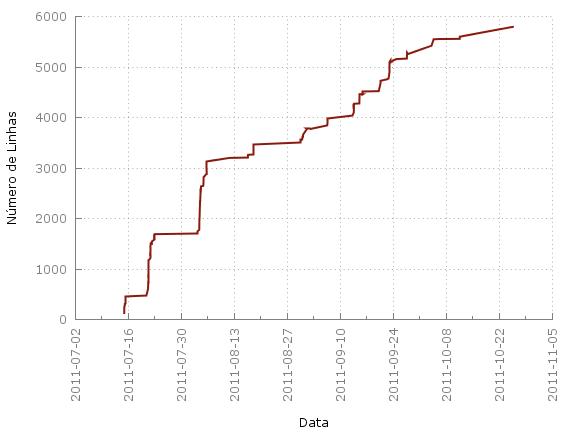
\includegraphics[width=0.7\textwidth]{./plots/lines_of_code.png}
	\caption[Evolução do número de linhas de código do projeto]{Evolução do número de linhas de código do projeto ao longo do processo de desenvolvimento}
	\fonte{Autoria Própria}
	\label{fig:linesofcode}
\end{figure}

\begin{figure}[!htb]
	\centering
	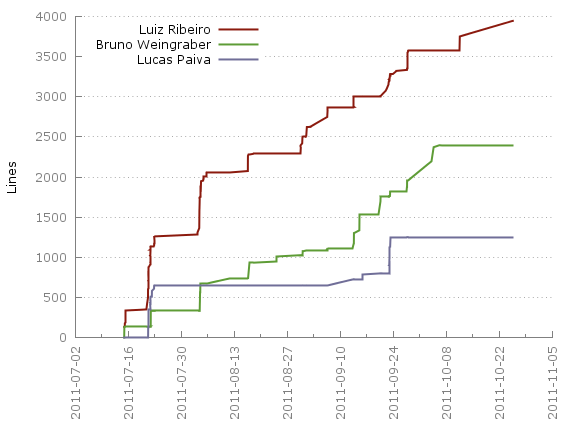
\includegraphics[width=0.7\textwidth]{./plots/lines_of_code_by_author.png}
	\caption[Evolução do número de linhas de código por programador]{Evolução do número de linhas de código do projeto por programador ao longo do processo de desenvolvimento}
	\fonte{Autoria Própria}
	\label{fig:linesofcodebyauthor}
\end{figure}

\begin{figure}[!htb]
	\centering
	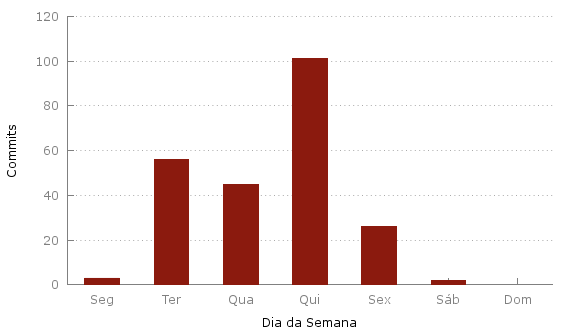
\includegraphics[width=0.7\textwidth]{./plots/day_of_week.png}
	\caption[Número de \emph{commits} por dia da semana]{Número de \emph{commits} por dia da semana}
	\fonte{Autoria Própria}
	\label{fig:dayofweek}
\end{figure}

\begin{figure}[!htb]
	\centering
	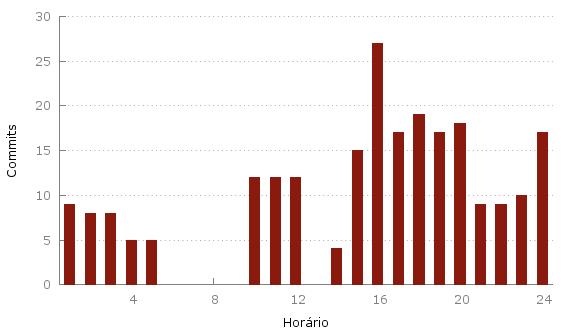
\includegraphics[width=0.7\textwidth]{./plots/hour_of_day.png}
	\caption[Número de \emph{commits} por horário]{Número de \emph{commits} por horário}
	\fonte{Autoria Própria}
	\label{fig:hourofday}
\end{figure}

\section{Performance do Serviço}

\begin{figure}[!htb]
	\centering
	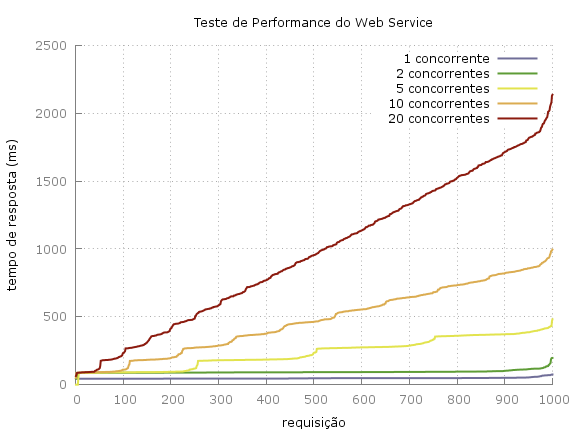
\includegraphics[width=0.7\textwidth]{./plots/stresstests/out.png}
	\caption[Tempo de resposta do \emph{Web Service}]{Tempo de resposta do \emph{Web Service} em função do número de requisições}
	\fonte{Autoria Própria}
	\label{fig:response}
\end{figure}

\section{Considerações}

% TODO
